\documentclass[a4paper]{article}
\usepackage{authblk}
\usepackage{graphicx}

% for code colouring
\usepackage{pgf,pgfarrows,pgfnodes,pgfautomata,pgfheaps,pgfshade}
\usepackage{amsmath,amssymb}
\usepackage[latin1]{inputenc}
\usepackage{colortbl}
\usepackage[procnames]{listings}
%%%%%%%%%%%%%%%%%%%%%

\usepackage{subfig}


\title{\texttt{Docker} \& \texttt{HENP}}
\author{S\'ebastien Binet}
\date{Novembre 2015}
\affil{CNRS/IN2P3/LPC}

\begin{document}
\maketitle

\section*{Introduction}
Le d\'eveloppement logiciel en physique des hautes \'energies -- en particulier
pour les exp\'eriences LHC -- met en jeu l'assemblage et l'int\'egration d'un
grand nombre de biblioth\`eques (externes ou internes, scientifiques ou
g\'en\'erales) qui doivent \^etre ensuite compil\'ees, test\'ees et install\'ees
sur les machines de production.

De plus, et \`a cause des ressources limit\'ees \`a disposition, les logiciels
des exp\'eriences ne sont test\'es et d\'eploy\'es que sur un jeu tr\`es
limit\'e de plateformes, architectures, cha\^ines de compilation et syst\`emes
d'exploitation.
M\'ecaniquement, l'installation d'un environnement de travail sur une machine de
d\'eveloppement avec un syst\`eme l\'eg\`erement diff\'erent
(Debian/CentOS/\ldots) ou bien sur une
machine de production exploitant une nouvelle architecture, est g\'en\'eralement
un processus it\'eratif chronophage, surtout lorsque les performances natives
(sans machine virtuelle) sont requises.

En effet, les machines virtuelles (\emph{VM}) ont grandement facilit\'e le
d\'evelop\-pement et le d\'eploiement d'applications d'une part, ainsi que la
gestion et l'optimisation de l'utilisation de \emph{clusters} de calcul d'autre
part.
Cependant, la virtualisation de l'environnement de travail s'est effectu\'ee au
prix de performances diminu\'ees par rapport aux performances natives.

Si les \emph{VM}s offrent un virtualisation au niveau d'une machine enti\`ere,
les conteneurs offrent quant \`a eux une virtualisation de l'environnement au
niveau du syst\`eme d'exploitation.
Les conteneurs semblent donc mieux r\'epondre aux besoins d'\texttt{HENP},
l'environnement de production \'etant essentiellement des clusters
\texttt{Linux}.
\texttt{LXC}~\cite{ref-lxc} et \texttt{OpenVZ}~\cite{ref-openvz} ont \'et\'e les
premiers \`a introduire les conteneurs dans l'\'ecosyst\`eme \texttt{Linux}, mais
\texttt{docker}~\cite{ref-docker} est le projet qui les a r\'eellement
popularis\'es et d\'emocratis\'es.

Cet article explore les possibles applications des conteneurs \texttt{docker}
aux environnements de travail typiques dans \texttt{HENP}.


%\section*{Origines}
\section*{Technologies utilis\'ees}

\texttt{Docker} est un projet \emph{open source} \'ecrit en
\texttt{Go}~\cite{ref-golang} pour empaqueter, distribuer et lancer n'importe
quelle application \`a l'int\'erieur d'un conteneur.

\begin{figure}[h]
\begin{center}
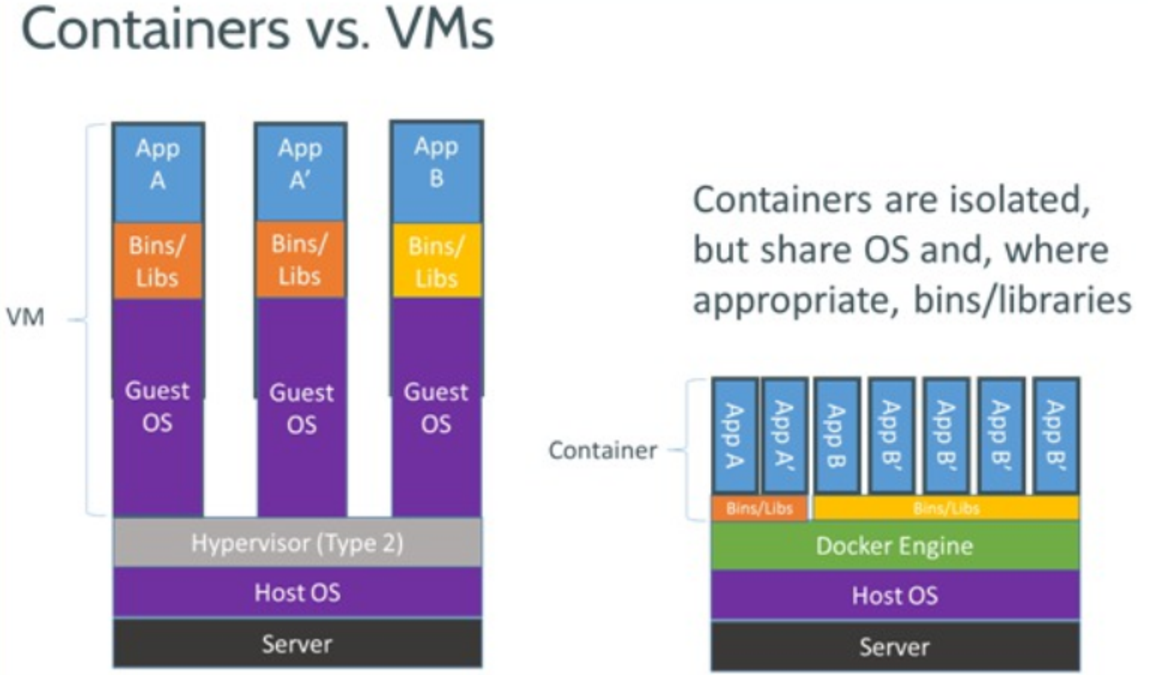
\includegraphics[width=0.8\linewidth]{figs/vm-lxc.pdf}
\end{center}
\caption{\label{fig-docker-overview}Comparaison entre machines virtuelles (\`a
	gauche) et conteneurs (\`a droite).
La virtualisation l\'eg\`ere \`a base de conteneurs repose sur le syst\`eme
d'exploitation pour l'isolation plut\^ot que de virtualiser tout le
mat\'eriel.}
\end{figure}
 
\texttt{Docker} utilise les espaces de nommage (\emph{namespaces})
\texttt{Linux}, les \texttt{cgroups}~\cite{ref-cgroups} et un syst\`eme de
fichiers permettant la fusion de points de montage (\emph{unioning}) pour isoler
les processus.
Les images de conteneurs sont similaires aux images de machines virtuelles, mais
partagent le noyau \texttt{Linux} avec la machine h\^ote.
Cette configuration met \`a disposition un syst\`eme plus l\'eger et permet de
provisionner des images de conteneurs en quelques secondes -- \`a comparer aux
plusieurs minutes pour les VMs -- mais permet \'egalement de lancer plusieurs
centaines de conteneurs sur une machine de bureau typique.

Gr\^ace aux \texttt{cgroups}, les conteneurs peuvent avoir leur propres
interfaces r\'eseau et sont famili\`erement vus comme un super-\texttt{chroot},
sans avoir recours \`a une quelconque \'emulation de materiel -- permettant
ainsi d'atteindre les performances optimales de la machine physique.
\texttt{docker} utilise \'egalement un syst\`eme de fichiers \`a plusieurs
couches \emph{via} un syst\`eme de fichiers d'\emph{unioning}
(\texttt{UnionFS}\cite{ref-unionfs}, \texttt{AUFS}~\cite{ref-aufs}) ou
\emph{via} \texttt{device mapper} pour les noyaux \texttt{Linux} sans cette
fonctionalit\'e.
Chaque couche du syst\`eme de fichiers est mont\'ee au dessus des
pr\'ec\'edentes.
La premi\`ere couche est appell\'ee \emph{image de base} et contient la
collection initiale de fichiers et r\'epertoires mis \`a disposition par une
distribution \texttt{Linux} donn\'ee (Ubuntu, RHEL, Fedora, etc\ldots),
distribution qui peut ne pas \^etre la m\^eme que celle install\'ee sur la
machine h\^ote.
Chaque couche est en lecture seule (seule la derni\`ere couche est modifiable)
et seules les diff\'erences avec la couche pr\'ec\'edente sont stock\'ees sur
disque.
Les diff\'erentes couches sont index\'ees \emph{via} un \emph{hash} \`a la
\texttt{git} et peuvent \^etre partag\'ees et r\'eutilis\'ees par diff\'erentes
images: cette strat\'egie permet d'optimiser les ressources de stockage et les
performances de provisionnement de disques.

\subsection*{Images \texttt{docker}}

Les images \texttt{docker} sont cr\'e\'ees \`a partir d'une image de base.
\texttt{Docker} met \`a disposition un nombre important d'images de base
officielles (\texttt{ubuntu}, \texttt{centos}, etc\ldots).
Ces images peuvent \^etre t\'el\'echarg\'ees \emph{via} la commande
\texttt{docker pull} comme illustr\'e dans la figure~\ref{fig-docker-pull}.

\begin{figure}[h]
\begin{lstlisting}[language=sh,
    basicstyle=\tiny,
    frame=trbl,
    numbers=left,
    showstringspaces=false,
    stringstyle=\ttfamily]
>> docker pull ubuntu
latest: Pulling from ubuntu
e9e06b06e14c: Pull complete 
a82efea989f9: Pull complete 
37bea4ee0c81: Pull complete 
07f8e8c5e660: Already exists 

Digest: sha256:8126991394342c2775a9ba4a843869112da8156037451fc424454db43c25d8b0
Status: Downloaded newer image for ubuntu:latest
\end{lstlisting}
\caption{\label{fig-docker-pull}\texttt{pull} t\'el\'echarge une image
	\texttt{docker} depuis le registre (aussi appel\'e \texttt{docker hub}).}
\end{figure}

La liste des images locales peut \^etre consult\'ee en lan\c cant la sous-commande
\texttt{docker~images}, comme montr\'e dans la figure~\ref{fig-docker-images}.

\begin{figure}[h]
	\begin{lstlisting}[language=sh,
		basicstyle=\tiny,
		frame=trbl,
		numbers=left,
		showstringspaces=false,
	stringstyle=\ttfamily]
>> docker images
REPOSITORY     TAG        IMAGE ID        CREATED             VIRTUAL SIZE
ubuntu         latest     07f8e8c5e660    5 days ago          188.3 MB
centos         latest     fd44297e2ddb    2 weeks ago         215.7 MB
ubuntu         12.10      c5881f11ded9    10 months ago       172.1 MB
\end{lstlisting}
\caption{\label{fig-docker-images}\texttt{images} affiche la liste des
	images locales, t\'el\'echarg\'ees depuis le \emph{hub} ou cr\'e\'ees
	localement.}
\end{figure}

Il est \'egalement possible to lancer des conteneurs en t\^ache de fond, le cas
typique \'etant les (micro)services, \emph{daemons} et serveurs web.
La syntaxe est donn\'ee dans la figure~\ref{fig-docker-run-detached}.

\begin{figure}[h]
	\begin{lstlisting}[language=sh,
		basicstyle=\tiny,
		frame=trbl,
		numbers=left,
		showstringspaces=false,
	stringstyle=\ttfamily]
>> docker run -d ubuntu sh -c 'while true; do echo "hello"; sleep 1; done;'
0ac942723c259a4963e0feff04d57e9bf8ad28e72158a231111d8f3718d960e6

>> docker ps
CONTAINER ID   IMAGE           COMMAND                CREATED         STATUS
0ac942723c25   ubuntu:latest   "\"sh -c 'while true   6 seconds ago   Up 3 seconds

>> docker attach 0ac942723c25
hello
hello
hello
hello
...
\end{lstlisting}
\caption{\label{fig-docker-run-detached}\texttt{docker run} en t\^ache de fond.
Ici, la commande \texttt{sh} est lanc\'ee dans un conteneur bas\'e sur l'image \texttt{ubuntu}.}
\end{figure}

Comme la commande est lanc\'ee en t\^ache de fond, il faut attacher les
E/S du terminal au conteneur (\texttt{0ac942723c25})
pour voir les messages s'afficher.
La gestion d'un conteneur peut \'egalement \^etre effectu\'ee \emph{via} les
sous-commandes \texttt{start/stop/restart}.

Les images \texttt{docker} peuvent \^etre consult\'ees, publi\'ees et
t\'el\'echarg\'ees depuis le \texttt{Docker Hub}~\cite{ref-docker-hub}: un
registre global d'images officielles et d'images cr\'e\'ees par la communaut\'e.
Cet index d'images peut \^etre consult\'e depuis la ligne de commande, comme
dans la figure~\ref{fig-docker-search}, ou bien depuis le web:
\texttt{https://hub.docker.com}.

\begin{figure}[h]
	\begin{lstlisting}[language=sh,
		basicstyle=\tiny,
		frame=trbl,
		numbers=left,
		showstringspaces=false,
	stringstyle=\ttfamily]
>> docker search apache
NAME               STARS     OFFICIAL   AUTOMATED
tomcat             131       [OK]       
tutum/apache-php   71                   [OK]
httpd              50        [OK]       
maven              32        [OK]       
fedora/apache      30                   [OK]
[...]

>> docker pull fedora/apache
Pulling repository fedora/apache
963668e7af33: Download complete 
963668e7af33: Pulling image (latest) from fedora/apache 
3d26c48a13f: Download complete 
Status: Downloaded newer image for fedora/apache:latest

>> docker run -d -p 80 fedora/apache
128d9712c922aab640a68d56c1cc35f5c17a889e136bc7983804035333264d92

>> docker ps
CONTAINER ID   IMAGE                  COMMAND             PORTS
128d9712c922   fedora/apache:latest   "/run-apache.sh"    0.0.0.0:32768->80/tcp

>> curl localhost:32768
Apache

\end{lstlisting}
\caption{\label{fig-docker-search}\texttt{docker search} consulte le registre,
	cherchant des images dont le nom ou la description contient la cha\^ine de
	caract\`eres demand\'ee.
	L'image \texttt{fedora/apache} expose un serveur web \texttt{Apache} sur le
	port \texttt{80} qui doit donc \^etre redirig\'e vers la machine h\^ote.
	\texttt{docker} peut se charger de faire la redirection vers un port ne
	n\'ecessitant pas de privil\`eges \texttt{root}.
}
\end{figure}

\subsection*{Cr\'eation d'images personnalis\'ees}
Un utilisateur peut cr\'eer de nouvelles images de mani\`ere interactive.
Pour cela, il lui suffit de:
\begin{itemize}
 \item lancer un conteneur \`a partir d'une image de base,
 \item lancer des commandes de mani\`ere interactive \`a l'int\'erieur du
	 conteneur,
 \item et de sauvegarder l'\'etat actuel du conteneur dans une nouvelle image,
\end{itemize}
comme montr\'e dans la figure~\ref{fig-docker-create}.

\begin{figure}[h]
	\begin{lstlisting}[language=sh,
		basicstyle=\tiny,
		frame=trbl,
		numbers=left,
		showstringspaces=false,
	stringstyle=\ttfamily]
>> docker run -i -t ubuntu bash
root@5ad62f3a9b4b:/>> apt-get install -y memcached
[...]
Unpacking memcached (1.4.14-0ubuntu9) ...
root@5ad62f3a9b4b:/>> exit
exit

>> docker ps -l
CONTAINER ID        IMAGE               COMMAND             CREATED
5ad62f3a9b4b        ubuntu:latest       "bash"              3 minutes ago

>> docker commit 5ad62f3a9b4b binet/memcached
220c5747349a7ec1e16297eec0df11eac277b9a9a6a149e386aff9f63bec868e

>> docker images
REPOSITORY          TAG           IMAGE ID            CREATED             VIRTUAL SIZE
binet/memcached     latest        220c5747349a        4 minutes ago       190 MB
ubuntu              latest        07f8e8c5e660        5 days ago          188.3 MB
centos              latest        fd44297e2ddb        2 weeks ago         215.7 MB
fedora/apache       latest        963668e7af33        2 weeks ago         627.1 MB
ubuntu              12.10         c5881f11ded9        10 months ago       172.1 MB
 
\end{lstlisting}
\caption{\label{fig-docker-create}\texttt{docker run} lance la commande
	\texttt{bash} dans le conteneur, en mode interactif (\texttt{-i}) avec un
	pseudo-terminal \texttt{TTY} (\texttt{-t}).
	Une fois que le conteneur est dans l'\'etat voulu (les paquets n\'ecessaires
	install\'es, les applications configur\'ees correctement, etc\ldots), il
	peut \^etre sauvegard\'e comme une nouvelle image, appel\'ee
\texttt{binet/memcached} dans cet exemple.}
\end{figure}

La cr\'eation d'images en interactif est tr\`es utile pendant le d\'eveloppement
ou le d\'ebogage du processus de cr\'eation.
Cependant, une interface de scriptage est n\'ecessaire pour la reproducibilit\'e
du processus de cr\'eation ainsi que pour son passage \`a l'\'echelle.
Le projet \texttt{docker} a donc introduit le concept du fichier
\texttt{Dockerfile} et d\'efini ses sp\'ecificit\'es.
Les fichiers \texttt{Dockerfile} sont ainsi l'\'equivalent des \texttt{Makefile}
pour la cr\'eation de nouvelles images.
La syntaxe de ces fichiers ressemble \`a celle des scripts shell, avec quelques
mots clefs list\'es et d\'ecrits par~\cite{ref-docker-dockerfile}.

Le fichier \texttt{Dockerfile} \'equivalent aux commandes de la
figure~\ref{fig-docker-create} est report\'e dans la
figure~\ref{fig-docker-dockerfile-create}.
La nouvelle image correspondant \`a la recette d\'ecrite par le fichier
\texttt{Dockerfile} est cr\'e\'ee en lan\c cant la commande
\texttt{docker~build} depuis le r\'epertoire contenant le fichier
\texttt{Dockerfile}.

\begin{figure}[h]
	\begin{lstlisting}[language=sh,
		basicstyle=\tiny,
		frame=trbl,
		numbers=left,
		showstringspaces=false,
	stringstyle=\ttfamily]
>> cat Dockerfile
## create a memcached image
FROM ubuntu
MAINTAINER me@example.com

RUN apt-get install -y memcached

>> docker build --tag=binet/memcached .
Sending build context to Docker daemon 2.048 kB
Sending build context to Docker daemon 
Step 0 : FROM ubuntu
 ---> 07f8e8c5e660
Step 1 : RUN apt-get install -y memcached
 ---> Running in 7f8349773ece
[...]
 ---> aac9f626b9fb
Removing intermediate container 7f8349773ece
Successfully built aac9f626b9fb

>> docker images
REPOSITORY          TAG                 IMAGE ID            CREATED              VIRTUAL SIZE
binet/memcached     latest              aac9f626b9fb        About a minute ago   190 MB
\end{lstlisting}
\caption{\label{fig-docker-dockerfile-create}Un exemple simple de fichier
	\texttt{Dockerfile}, scriptant la creation d'une nouvelle image \`a partir
	de l'image \texttt{ubuntu}, dans laquelle l'application \texttt{memcached}
est install\'ee.}
\end{figure}


\section*{Cas d'usages}

\texttt{Docker} est tr\`es utile pour un certain nombre de \emph{workflows}
typiques dans \texttt{HENP}.
\texttt{Docker} permet en effet:
\begin{itemize}
 \item l'encapsulation de la construction de l'enti\`eret\'e de la pile
	 logicielle d'une exp\'erience, en s'assurant qu'il n'y a aucune
	 d\'ependance externe implicite cach\'ee,
 \item l'installation et le d\'eploiement d'une pile logicielle d\'ej\`a
	 compil\'ee sur un nombre arbitraire de n\oe uds et de sites, ainsi qu'une
	 rapide mise en production de cette pile logicielle,
 \item la distribution simple et rapide d'environnements de d\'eveloppement.
\end{itemize}

\texttt{Docker} permet \'egalement une r\'epartition plus souple des
responsabilit\'es entre les \'equipes de d\'eveloppement et de production, en
ad\'equation avec la mouvance \emph{DevOps}~\cite{ref-devops}.

L'\'equipe de d\'eveloppement peut ainsi choisir la distribution \texttt{Linux}
ad\'equate, le portefeuille de d\'ependances externes (ainsi que leur version),
son cadriciel, etc\ldots sans impact pour l'\'equipe de production (autre que
l'adoption des conteneurs comme outil de mis en production).
De son c\^ot\'e, l'\'equipe de production peut se focaliser sur la gestion des
machines, la gestion des logs, la politique de sauvegarde des donn\'ees, le
\emph{monitoring}, etc\ldots sans interf\'erer avec le processus
de d\'eveloppement.

Dans cette optique, un certain nombre d'images de bases ont \'et\'e cr\'e\'ees
sp\'ecifiquement pour la communaut\'e \texttt{HENP} et ont \'et\'e collect\'ees
dans le d\'ep\^ot \texttt{github.com/hepsw/docks}.
Entre autres:
\begin{itemize}
	\item \texttt{Scientific Linux CERN 5} (\texttt{hepsw/slc5-base}),
	\item \texttt{Scientific Linux CERN 6} (\texttt{hepsw/slc-base}) et,
	\item \texttt{CERN CentOS 7} (\texttt{hepsw/cc7-base}).
\end{itemize}

Dans ce d\'ep\^ot se trouvent \'egalement les fichiers \texttt{Dockerfile}
n\'ecessaires pour la cr\'eation d'images contenant l'installation binaire du
cadriciel \texttt{Gaudi}~\cite{ref-gaudi} (\texttt{hepsw/lhcb-gaudi}) et la
suite logicielle d'analyse de l'exp\'erience LHCb, \texttt{Da Vinci}
(\texttt{hepsw/lhcb-davinci}).
Ces images n'ont cependant pas \'et\'e publi\'ees sur le \texttt{Docker Hub} \`a
cause de leur taille ($O(10 GB)$).
Il serait sans doute int\'eressant d'avoir un \emph{hub} d\'edi\'e \`a la
communaut\'e \texttt{HENP}, g\'erant de fa\c con transparente les certificats
grilles.

Ce d\'ep\^ot sert \'egalement des images contenant le d\'emon \texttt{CVMFs}
correctement install\'e, configur\'e et pr\^et \`a distribuer la pile logicielle
de diff\'erentes exp\'eriences (ATLAS, CMS, LHCb et LSST).

\section*{Conclusions et perspectives}
Cet article a pr\'esent\'e \texttt{docker} et quelques unes des applications
possibles dans la communaut\'e \texttt{HENP}.
La \emph{"conteneurisation"} de piles logicielles \texttt{HENP} est faisable et
devrait se g\'en\'eraliser et s'acc\'elerer dans le futur.
Les conteneurs ne pr\'esentent pas de performances d\'egrad\'ees par rapport aux
performances natives, et ce, m\^eme pour des applications gourmandes en
\emph{CPU} et \emph{E/S}~\cite{ref-bench-0,ref-bench-1}.
De plus, \texttt{docker} (ou tout autre technologie de virtualisation
l\'eg\`ere) peut potentiellement faciliter l'optimisation de l'utilisation des clusters de calcul
\texttt{Linux}, sans avoir recours aux machines virtuelles.

Un autre usage int\'eressant de conteneurs est l'empaquetage d'application (et
ce sans couplage avec le gestionnaire de paquets de la distribution
\texttt{Linux} sous-jacente) ainsi que la preservation des donn\'ees et de la
pile logicielle d'une exp\'erience, permettant la r\'e-analyse ou la
r\'e-interpretation des r\'esultats plusieurs ann\'ees apr\`es la fin de cette
exp\'erience.

Le paysage de la virtualisation l\'eg\`ere est encore en pleine \'evolution et
maturation.
Des initiatives telles qu'\texttt{appc}~\cite{ref-appc}, une standardisation du
format de conteneurs pour une meilleure interoperabilit\'e, lanc\'ee par un
concurrent de \texttt{docker}, \texttt{rkt}~\cite{ref-rkt}, ou bien
\texttt{oci}~\cite{ref-oci}, l'\emph{Open Container Initiative}, sont \`a
surveiller.
En effet, \texttt{rkt} semble en bonne voie de concurrencer fortement \texttt{docker} sur
le front de la s\'ecurit\'e, ayant un code moins monolithique (et plus
facilement auditable, avec des privil\`eges plus restreints) que ce
dernier.

Une saine comp\'etition semble s'engager entre les diff\'erents acteurs de la
virtualisation l\'eg\`ere et devrait profiter \`a la communaut\'e.

\begin{thebibliography}{9}

	\bibitem{ref-golang} \texttt{Go},
		\verb'https://golang.org'

	\bibitem{ref-docker} \texttt{Docker},
		\verb'http://docker.io'

	\bibitem{ref-docker-hub} \texttt{Docker} Hub,
		\verb'https://hub.docker.com'

	\bibitem{ref-docker-dockerfile} \texttt{Dockerfile} syntax reference,
		\verb'https://docs.docker.com/reference/builder'

	\bibitem{ref-lxc} \texttt{LXC},
		\verb'https://linuxcontainers.org'

	\bibitem{ref-openvz} \texttt{OpenVZ},
		\verb'https://openvz.org'

	\bibitem{ref-cvmfs} \texttt{CernVM} File System,
		\verb'http://cernvm.cern.ch/portal/filesystem'

	\bibitem{ref-cgroups} \texttt{Linux} control groups,
		\verb'http://en.wikipedia.org/wiki/Cgroups'

	\bibitem{ref-boot2docker} \texttt{boot2docker}, a lightweight \texttt{Linux}
		distribution to run \texttt{docker} containers,
		\verb'http://boot2docker.io/'

	\bibitem{ref-bench-0} \texttt{KVM} and \texttt{docker} benchmarking,\\
		\verb'http://bodenr.blogspot.ch/2014/05/kvm-and-docker-lxc-benchmarking-with.html'

	\bibitem{ref-bench-1} Felter W. et al., "An Updated Performance Comparison of Virtual Machines
		and Linux Containers", RC25482, 2014

	\bibitem{ref-gaudi} Barrand G. et al., "\texttt{GAUDI} -- A software architecture and
		framework for building LHCb data processing applications",
		CHEP 2000

	\bibitem{ref-appc} App Container Specification and Tooling,\\
		\verb'https://github.com/appc/spec'

	\bibitem{ref-oci} The Open Container Initiative,\\
		\verb'https://www.opencontainers.org'

	\bibitem{ref-rkt} \texttt{rkt}, an App Container runtime for
		\texttt{Linux},\\
		\verb'https://github.com/coreos/rkt'

	\bibitem{ref-jenkins} Jenkins, an extensible open source continuous
		integration server,
		\verb'https://jenkins-ci.org/'

	\bibitem{ref-mesos} Mesos, a distributed systems kernel,
		\verb'http://mesos.apache.org/'

	\bibitem{ref-unionfs} UnionFS, A Stackable Unification File System,\\
		\verb'http://unionfs.filesystems.org/'

	\bibitem{ref-aufs} AuFS, advanced multi layered unification filesystem,\\
		\verb'http://aufs.sourceforge.net/'

	\bibitem{ref-devicemapper} device mapper,
		\verb'http://www.sourceware.org/dm/'

	\bibitem{ref-devops} DevOps,
		\verb'http://en.wikipedia.org/wiki/DevOps'

\end{thebibliography}


\end{document}
